% !TeX spellcheck = en_GB
\section{Introduction}
During the last years the usage of smart-wearables (particularly smartwatches) has become more and more common with a number of 337 million units sold in 2019 and a forecast in sales of up to 527 million units by 2024 \cite{tenzer}.
With that also comes a natural demand in data protection caused by the amount of sensors built in these devices and their ability to capture sensible personal data (e.g. health informations).
Additionally smart devices can now also be used for many kinds of financial actions.
Since most wearables are connected to either the distributors or the respective mobile phones virtual assistant they should contain sensors for on one hand sound conduction and on the other hand audio recording.
In the current general smart-wearable design neither of these sensors is oriented towards the wearers arm.
With a change in position of these sensors smartwatches become eligible for functional biometric authentication.
Further motivation for this new authentication method comes from the fact that the previous classical methods (PIN, password...) are not suited for usage on smartwatches \cite{xu2017gait}.   
Nevertheless it is shown by Johnston \cite{johnston2015smartwatch} and Yang \cite{yang2015motionauth} in their respective works that there already are potential biometric authentication methods for smartwatches based on distinct hand or arm movements. 

From these preconditions a prototype is defined. This prototype uses a sound based functional biometric which gets applied to its wearers arm. 

\section{Related Work}
This section will give an overview on the terms of biometrics and its variations, authentication and also what defines an authentication system.
Additionally an insight into other works on biometric or smartwatch based authentication will be provided. 

\subsection{Authentication}
The term in general describes the process based on which a security systems tries to approve someone's claim of identity \cite{bhattacharyya2009biometric}.
Based on the input type of this claim the term authentication can be further subdivided into explicit and implicit authentication.
\textit{Explicit} authentication is more often also known as traditional authentication \cite{ranjan2016automatic}.
This includes providing knowledge like PIN or password, using a token but also performing gestures, fingerprints etc. from the biometrical field.

\textit{Implicit} authentication on the other hand describes mechanisms where a user does not provide a password, etc. directly.
Instead users are authenticated based on observations of their behavioural patterns\cite{jakobsson2009implicit}.
These observations are qualified for the use in e.g. biometrics since every individual has its own distinct habits which could be captured and analysed using different sensors \cite{shi2010implicit}.
Furthermore Shi, Jakobsson et al. state in their 2009 and 2010 works that implicit authentication is well suited for usage in combination with mobile smart-devices \cite{shi2010implicit} or portable computers \cite{jakobsson2009implicit}.
Based on this they propose three different application scenarios.
First as a second factor in combination with passwords, second as the main authenticator and thus replacing the usage of a password and last as additional assurance or an extra trust factor when performing e.g. financial actions on a mobile device.

\subsection{Biometrics}
\textit{Biometrics} (as in the Greek terms \textit{bios} and \textit{metrikos}) describes the utilization of an individuals physical traits or behaviour to clearly identify one from others. Contrary to the more known verification methods of PINs, passwords or ID-cards biometric identification does not rely on tokens or knowledge which could easily be forgotten or stolen, rather than unique personal traits like fingerprints, face geometry or the specific way someone interacts \cite[chpt. 1.1]{jain2007handbook}\cite{delac2004survey}.
Depending on the concept of usage a biometric system can be used in either verification or identification mode \cite[chpt. 1.3]{jain2007handbook}.
These two modes can also be differed by the use of \textit{positive} or \textit{negative identification} techniques \cite{wayman2005introduction}.

As already stated above biometric authentication uses an individuals personal traits as authentication tokens. Based on the kind of trait and the methods how they are provided the general term of biometrics can be further divided into behavioural and physiological biometrics.
Also a new kind of biometrics called functional biometrics was introduced by Liebers and Schneegass in 2020 \cite{schneegass2020functbiometric}.

\subsubsection{Behavioural Biometrics}
Behavioural biometrics refers to authentication systems in which the process of authentication is related to the behaviour of an individual \cite{bhattacharyya2009biometric}.
In most cases this process is conducted with the use of primarily gestures or other actions or movements capable of being performed in everyday life \cite{yampolskiy2008behavioural}.
Features which can be used for behavioural biometrics include e.g gait, keystrokes but also authentication patterns on smartphones could be used.
One main advantage compared to physiological biometrics is that some behavioural traits must not be collected actively but can be captured whilst performing any kind of different tasks \cite{yampolskiy2008behavioural}. 
Also there is no definite need for special hardware since the sensors needed are mostly built in smart wearables which are one of the main users of behavioural biometrics \cite{johnston2015smartwatch}.

\subsubsection{Physiological Biometrics}
Apart from behavioural biometrics the classification of physiological biometrics is also existent. 
This form of biometric authentication uses the more "static" traits of a users body as token such as e.g. fingerprints, hand geometry \cite{alsaadi2015physiological} or vein patterns \cite{faltaous2019vpid}.

A physiological system should also have a little higher accuracy than a behavioural one and it should be harder to use as an imposter since it is nearly impossible to identically copy a finger print, iris pattern, etc. \cite{koong2014user}, \cite{delac2004survey}.

\subsubsection{Functional Biometrics} With functional biometrics another novel kind of biometric authentication was introduced lately by Liebers and Schneegass \cite{schneegass2020functbiometric}.
This new concept stands as a major influence to this work notably with its first implementation in SkullConduct\cite{SkullConduct}. 
\begin{figure}
	\begin{center}
		\subfloat[Traditional Biometrics]{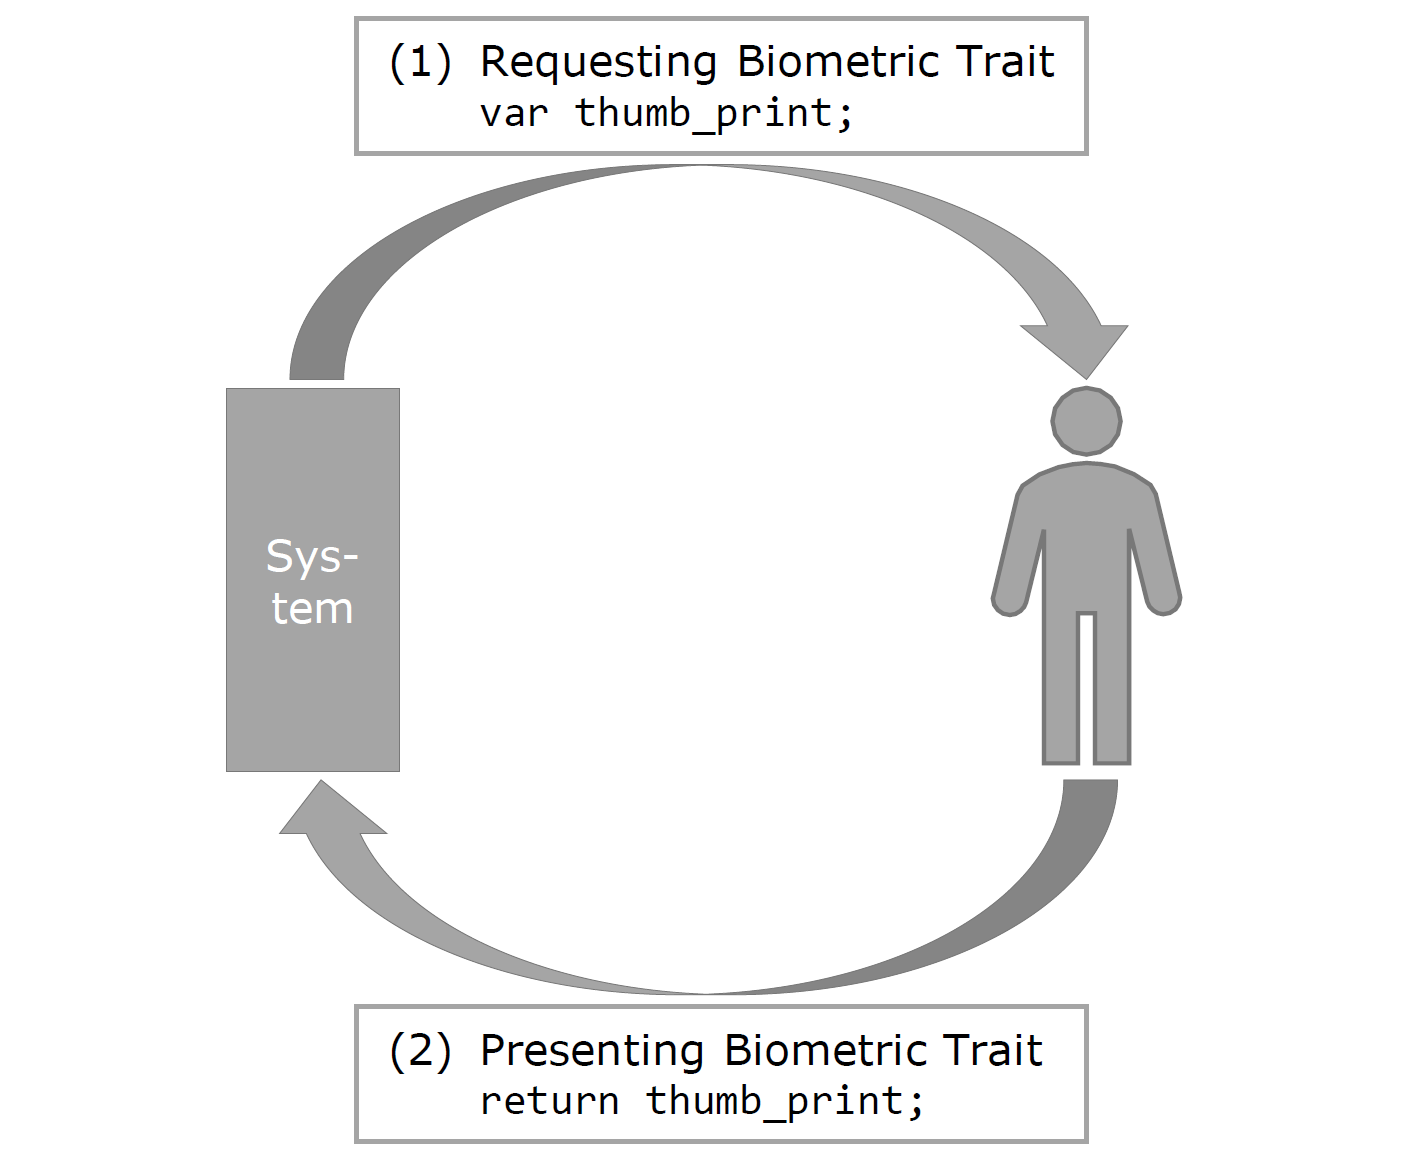
\includegraphics[width=0.4\textwidth]{Media/biometric_trad.png}\label{fig:tradBiom}}
		\hspace{0.5cm}
		\subfloat[Functional Biometrics]{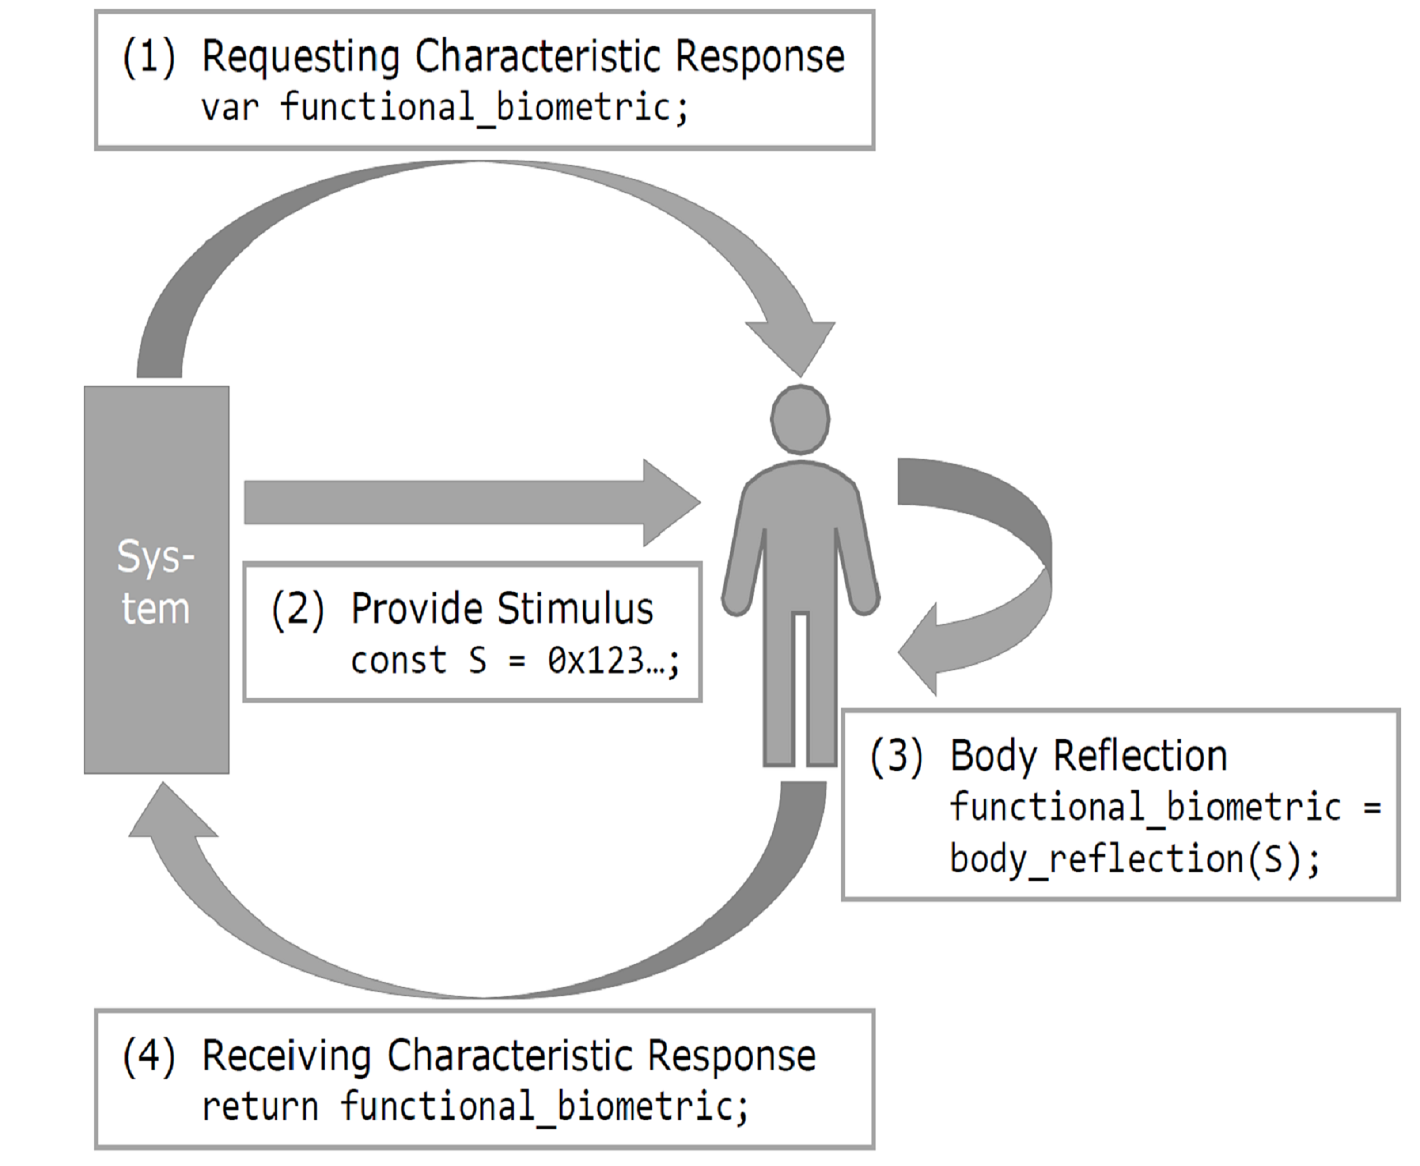
\includegraphics[width=0.4\textwidth]{Media/biometric_funct.png}\label{fig:functBiom}}
	\end{center}
	\caption{(a) shows the authentication process of a traditional biometric system where a characteristic response is created based on someone's unique trait.
	(b) shows the order of steps for functional biometrics when a stimulus is added to create the characteristic based on body reflections \cite{schneegass2020functbiometric}.}
	\label{fig:biometricsVersions}
\end{figure}

In this category of biometric authentication the authentication system provides an additional stimulus during the enrolment phase.
This stimulus is applied to the individuals body where it gets modified and afterwards captured (cf.~Figure~\ref{fig:functBiom}).
Due to different personal biological characteristics the modification of the stimulus is unique for each combination of user and stimulus.
Requirements Schneegass et al. proposed are two hardware components in form of a Stimulus Generation Unit (SGU) and a Body Reflection Sensor (BRS).
These two have to be designed as a dependence of the underlying biometric trait. Exemplarily when sound is used as the stimulus the SGU will be most likely some kind of microphone and the BRS a speaker.
During the enrolment process described above stimulus and its transformation are saved as a secret two-tuple ($x, f(x)$) with $ x $ being the stimulus and $ f(x) $ the transformation.
Now when the related user wants to authenticate the stimulus is reapplied and it is expected to get $f(x)$ as response again.
An additional security measure provided by functional biometrics is that when the stimulus gets leaked or lost the system is not fully compromised because the stimulus is only an exchangeable medium.
The secret stems from the body reflection function which is unique to the user, unknown and hard to manipulate.


As already mentioned before the SkullConduct work by Schneegass et al. is one of the key influences to this work. Not just because it is one of the first realizations for functional biometrics but it also 
serves as a source of inspiration for this work.
Schneegass et al. implemented a biometric authentication system using eyewear computers (e.g. Google Glass).
Therefore they used the concept of bone conduction which is already frequently used by hearing aids. SkullConduct, in this case, uses the bone conduction speaker of the Google Glass to emit a sound sample against the wearers head.
The sample which gets transformed due to the unique nature of each individuals head is captured by the glasses integrated microphone.
Results of this study  indicate that with all tested users SkullConduct had a probability of around 97\% when it comes just to identify a correct user.
Test of the system as an authentication tool showed an Equal Error Rate (EER) of around 6.9\% in average but with significant drops the shorter the used sample gets (less than 1 second).

Other work on authentication via smart devices includes e.g. the works from A. Johnston et al. who implemented a smartwatch based authentication module that used gait recognition \cite{johnston2015smartwatch}.
They adapted from previous work of theirs where gyro- and acceleration-sensors of smart phones were used to develop authentication methods \cite{kwapisz2010cell}.
The main thought behind the proposed use of gait authentication on smartwatches is that their place of wearing/usage is more consistent than the one of a smart phone and therefore more advantageous.
Each participants dataset includes both data from gyro- and acceleration-sensor.
Tests in regard of both design types showed that the general performance of authentication is way higher in average than the one of identification (e.g. 97.2\% compared to 79.2\%).
Additionally the overall performances of the acceleration-sensor was higher than the gyro-sensor.
Conclusions Johnston et al. drew from their results were that it is possible to authenticate someone sufficient enough using a smartwatch but they propose not to use the system for something other than a multi-modal biometric system at its current level. 
\newpage

\section{Concept}
With the introduction of functional biometrics, space was created for the development of new mechanisms and variations in biometric authentication.
Contrary to other biometric systems which rely on e.g. fingerprints the body function used in functional biometrics can not be leaked or reproduced that easily.
This is due to the function being comprised of each individuals own body structure and bone density \cite{schneegass2020functbiometric}.

A function based biometric system authenticates its user by applying a stimulus to the users body.
Based around the name-giving body-function a characteristic transformation of the stimulus happens which can be measured.
This measurement can then be compared with a previously stored measurement using the same stimulus to authenticate the user.

An already existing implementation approach to functional biometrics is the SkullConduct head mounted device (HMD) introduced by Schneegass et al. \cite{SkullConduct}.
There the stimulus used consisted of a sound sample being applied and re-captured by the HMD.
One limitation coming with this exemplary work is, that with the authentication being reliant on the HMD it is based around a device with rather fixed location.

From this point of view it would be more useful to have a device in smaller shape e.g. the form of a bracelet, which could be worn on either arms or legs.
It's functionalities could exemplarily be integrated into a smartwatch or other small wearable smart-devices. 
The authentication provided by the bracelet could be either used to secure data saved on the smart device or as multiple factor authentication for other connected devices like smartphones.

Possible stimuli for the bracelet could be sound patters which use either white noise, frequency changes or little melodies.
The stimulus can then be applied to the wearer on a regular basis over the time the device is worn to ensure it is used by the correct user.
Also, if the stimulus used gets leaked or corrupted otherwise, a functional biometric system does not need to be recalibrated completely.
Since even the system itself does not really know the nature of the transformation function only a new stimulus and new sample data are needed.

The prototype realised in this work consists of a microcontroller which is used to generate and apply the stimulus as well as to capture the transformation.
For this purpose it is connected to each a little microphone capsule and a speaker with small form factor.

\section{Implementation}
\subsection{Hardware}
\subsubsection{Components}
The microcontroller used in this project is the LoRa 32 by Heltec Automation\footnote{LoR Controller,~\url{https://heltec.org/project/wifi-kit-32/}}.
The controller uses an 32bit dual-core microprocessor by espressif (ESP32).
Other features include onboard Wi-Fi and Bluetooth as well as an 0.97 inch OLED display.
The controller can be powered using a micro-USB connection to a computer or an attachable lithium battery.

The implementation for the recordings is based around the use of an omnidirectional digital microphone\footnote{Ambility~INMP441,~\url{https://www.amazon.de/Ambility-Omnidirektionales-\\Mikrofonmodul-I2S-Schnittstelle-Precision/dp/B07MW95PSS}}.
This microphone uses a digital I$^{2}$S-Interface to process its input. 
For the output of the generated stimuli a miniature speaker with a mylar-membrane\footnote{LSF-15M/S,~\url{https://www.conrad.de/de/p/lsf-15m-s-8-ohm-0-8w-miniatur-\\lautsprecher-geraeusch-entwicklung-85-db-0-500-w-1-st-710277.html}} is used.
The speaker can conduct noise at up to 85~dB.
Further used hardware includes an SD-Card Reader equipped with an 32 Gigabyte SD-Card which is used to store the generated audio-samples.

An overview of the connection between controller and the other components can be seen in Figure~\ref{fig:pinout}.
An exact mapping of the single components can be taken from the code\footnote{URL zum Git einfügen}.
\begin{figure}[H]
	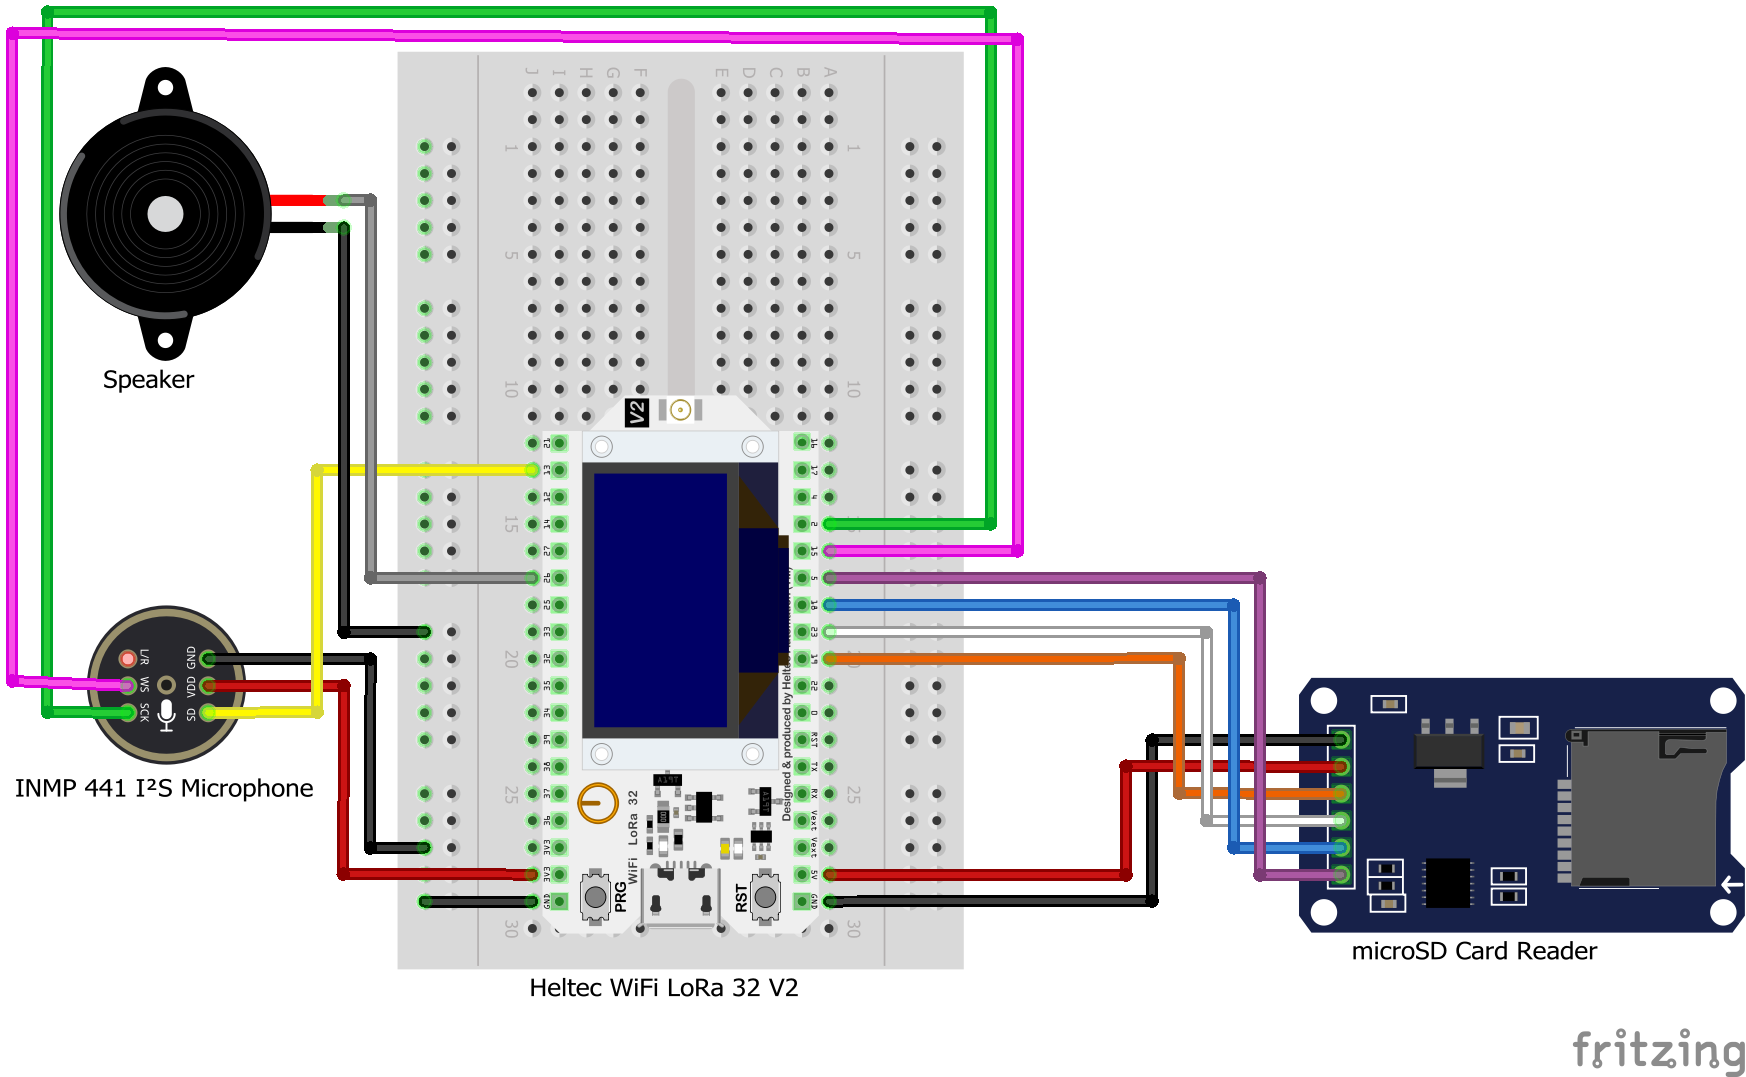
\includegraphics[width=\linewidth]{Media/Hardware_Pinout.png}
	\caption{Pinout scheme of every component used in the project. The battery-pack which can be connected to the underside of the controller is not shown here for reasons of clarity.}
	\label{fig:pinout}
\end{figure}
The hardware is powered by a lithium-ion battery with a capacity of 1200mAh and an output of 3.7V.
It is connected to the controller on its underside using a JST-PH connector. 

\subsubsection{Casing}
To conduct the associated study, where it is necessary to wear the hardware on the body, a case which is approximately shaped like a bracelet is designed.
The case consists of two major parts, one to store the controller and battery, the other containing microphone and speaker.
To keep the cases in place when in use they were fitted with a wristband made from stretchable rubber.
//TO BE CONTINUED....

%\subsection{Software}
%The following section will focus on every aspect regarding the development of the software used for this work.
%This includes the tools used (such as development environments or software to design the hardware-casing) but also the steps taken to design the actual %software are described. 
\subsection{Development Tools}
The majority of code in this project was written in the Arduino development environment (IDE). 
This open-source IDE is designed and optimized for the use with microcontrollers from the arduino family.
It is also possible to add plugins for the support of other microcontroller chips like ESP32 or the Heltec LoRa-controller.
Therefore it is necessary to include the functionality-packages provided by the chip developers under \texttt{"Tools > Board > Board Manager"} in the Arduino IDE.
The IDE supports C and C\texttt{++} as additional programming languages which can be processed by the microcontrollers.

Another major feature of the IDE is its ability to not only compile the designed sketches but also to flash them onto a microcontroller plugged into the computer via usb.

For the design of the casing the software Fusion 360 published by Autodesk was used.
With this CAD-software it is possible to design shapes in either 2D or 3D format.
These shapes can then be exported from Fusion 360 in a format which is readable by either a 3D-printer or laser-cutter.
 

\begin{figure}[H]
	\includegraphics[width=\linewidth]{Media/Controller_setup.png}
	\caption{Individual steps the microcontroller executes during its setup ordered as Statechart.}
	\label{fig:cntrlr_stp}
\end{figure}

\subsection{Software}
The code in this project is split up into multiple (logical) parts - the main .ino-file and additional .cpp files providing further code needed.
The main file locates the default microcontroller functions as well as functionalities to generate the audio stimulus.

As seen in Figure~\ref{fig:cntrlr_stp} the setup functions main focus lays on initializing the different hardware components and hosting the socket for the provided web server.
From this web server an interface is accessible which can be used to apply the stimulus and record its alterations.
To capture the recordings the i2s interface is used.

Information needed by the user can be printed onto the controllers OLED display.
For this purpose Heltec's version of the SSD1306 Library, which is included in the \enquote{\texttt{heltec.h}} package\footnote{\url{https://github.com/HelTecAutomation/Heltec_ESP32/blob/master/src/heltec.h}}, is needed.
It is located in the data included with the Heltec ESP32 board manager.
The packages functionalities are accessible by including its header at the beginning of the sketches main-file.

To print something onto the display it is necessary to use the following statements first line:
\begin{lstlisting}[style=inText]
	Heltec.display->drawString(int x, int y, String text);
	Heltec.display->display();
\end{lstlisting}
The parameters \texttt{x} and \texttt{y} represent the coordinates on the display starting on the top-left from where the string is to be printed and text being the content to be printed.
Afterwards the method \texttt{display()} has to be called using the  statements second line since just using the \texttt{drawString} method will only write the strings into a buffer but not print them onto the
display.
It is not necessary to call the method \texttt{display()} after each line but just once per block.

An additional feature which is implemented during the setup function is the connection to an NTP-Server.
This server is later used to uniquely identify the recorded data by adding date- and timestamps of the recordings start to each file.

\subsubsection{Stimulus Generation}
As for the stimulus' generation the used \texttt{tone()} function is implemented separately since the ESP32 chipset does not support its functionalities naturally.
For this purpose the LED PWM functions can be used.
Using this functionality it is possible to control and alter both frequency and duty cycle of the output.

Initially these values are set within the \texttt{ledcSetup()} function.
When changing the duty cycle at constant frequency it is possible to shift the pitch of the sound using the \texttt{ledcWrite()} function.
When changing the frequency at constant duty cycle it is possible to generate different notes.
To do so the function \texttt{ledcWriteTone()} has to be used instead of \texttt{ledcWrite()}.
\begin{lstlisting}[frame=single, language={c++}, style=style,
				   caption={Function used to generate a single note using frequency and sound duration.}, label={lst:toneFunct},float=!htb]
void tone(int channel, int frequency_in_HZ,
		  		long durance_in_ms) {

	long delayAmount = (long)(1000000 / frequency_in_HZ);
	long loopTime = (long)((durance_in_ms*1000) / 
												 (delayAmount*2));

	for (int x = 0; x < loopTime; x++) {
		ledcWriteTone(channel, 3000);
		delayMicroseconds(delayAmount);
		ledcWriteTone(channel, 0);
		delayMicroseconds(delayAmount);
	}
	delay(20);
}
\end{lstlisting}

Based on these conditions the function \texttt{tone()} as seen in Listing~\ref{lst:toneFunct} uses the method \texttt{ledcWriteTone()} to generate sound\footnote{The function is taken from the gitHub provided by André Tagliati~\cite{tagliati} and altered slightly to work with the ESP32 chipset.}.
Additionally the parameters \texttt{channel, frequency} and \texttt{durance} are required.
Using these parameters the function can determine the values for delay and loopTime representing pitch and sound duration respectively of the generated audio.
The third parameter is used to represent the PWM channel through which the sound will be forwarded.

Within the for-loop the \texttt{ledcWriteTone()} function is used to alternately set the PWM pin to high and low.
Between these alterations the pitch is set by setting a delay as previously computed.
As a final step a delay of 20 ms is set to separate the individual tone blocks from one another.

Now the actual stimulus can be designed by implementing a method which uses a combination of the tone-function as described above and the delay-function.
The method containing the stimulus can then be called during the loop-function each time a new recording is started through the web-interface.

\subsubsection{Recording the Sample}
With Inter-IC Sound (I$^2$S) an serial interface is used to generate the recordings needed for the study.
I$^2$S works with a bus consisting of minimum three lines.

The lines which are mandatory include Serial Clock (SCK), Word Select (WS) and Serial Data (SD) but it is also possible to add further lines to the bus.  

To work with an arduino or ESP32 based microcontroller it is necessary to include the I$^2$S-Drivers into the source-code.
Based on this package the methods\texttt{ i2sInit()}, \texttt{i2s\_adc\_data\_scale()} and \texttt{i2s\_adc()} operate.

Within \texttt{i2sInit()} the parameters needed by the I$^2$S framework are configured.
Also the ports needed by the hardware are assigned and it is defined whether sound shall be recorded (the serial data param is set to \texttt{data\_in\_num}) or emitted (the serial data param is set to \texttt{data\_out\_num}).

The actual recording-process is controlled by the method \texttt{i2s\_adc()}.
There the input form the microphone is captured using the method \texttt{i2s\_read()} from the I$^2$S package.
It is used to read the data captured by e.g. a microphone into a predefined destination address.
After defining the different buffer sizes needed during the recording process the input from the attached microphone is read and saved to a file.
This process takes until a specified file size is reached.
The file size is computed from amongst other parameters the sample rate, bits per sample but also the recordings duration.  

Since the natural volume of the recording is relatively low when using only the \texttt{i2s\_adc()} method each chunk of data can be scaled using the method \texttt{i2s\_adc\_data\_scale()} before writing it to the filesystem.
This scaling is done by multiplying each bit of the recording with a special factor as it can be seen in Listing~\ref{lst:adcScale} after performing a bitshift on the original values.
\begin{lstlisting}[frame=single, language={c++}, style=style,
	caption={The function which is used to scale the captured recordings volume.}, label={lst:adcScale},float=!htb]	
	void i2s_adc_data_scale(uint8_t* d_buff, uint8_t* s_buff, uint32_t len) {
		uint32_t j = 0;
		uint32_t dac_value = 0;
		
		for (int i = 0; i < len; i += 2) {
			dac_value = ((((uint16_t) (s_buff[i + 1] & 0xf) << 8)
						 | ((s_buff[i + 0]))));
			d_buff[j++] = 0;
			d_buff[j++] = dac_value * 256 / FACTOR;
		}
	}	
\end{lstlisting}
The parameter which is represented by the placeholder "FACTOR" in the Listing~\ref{lst:adcScale} is a multiple of 1024 where the less the value is set the louder the recording will become (For this implementation the value 4096 is used).
One little disadvantage of this method is that not only the recorded sound will be scaled but also the volume of other recorded noise is enhanced.

\subsubsection{Webinterface}
To manage the functions of this project and start the recordings and playbacks a webinterface is used.
It's implementation is located in the main .ino-file as a part of the loop-function.

As it can be seen in Listing~\ref{lst:WiFiCon} the socket listens for incoming clients and then processes the incoming requests as long as the client is connected.
The first response sent to an incoming client is "HTTP/1.1 200 OK" and the content-type of the response.

Additionally to this response code the client can process incoming GET-requests, e.g. when the button to start a recording is pressed on the webinterface.
For this handling if statements like the following are used.
\begin{lstlisting}[style=inText] 
	if (header.indexOf("GET /recording") >= 0) {...}  
\end{lstlisting}
The last mandatory feature which is printed to the client during this first if-statement consists of several single \texttt{client.println()} statements containing the data for the web page.
These prints have to go in between the last printed blank line (seen in line 25 of cf.,~Listing~\ref{lst:WiFiCon}) and the if-statements to handle incoming requests as described above.

How the webinterface is displayed is shown in Figure~\ref{fig:webinterface} using the browser Microsoft Edge.
\begin{figure}
	\frame{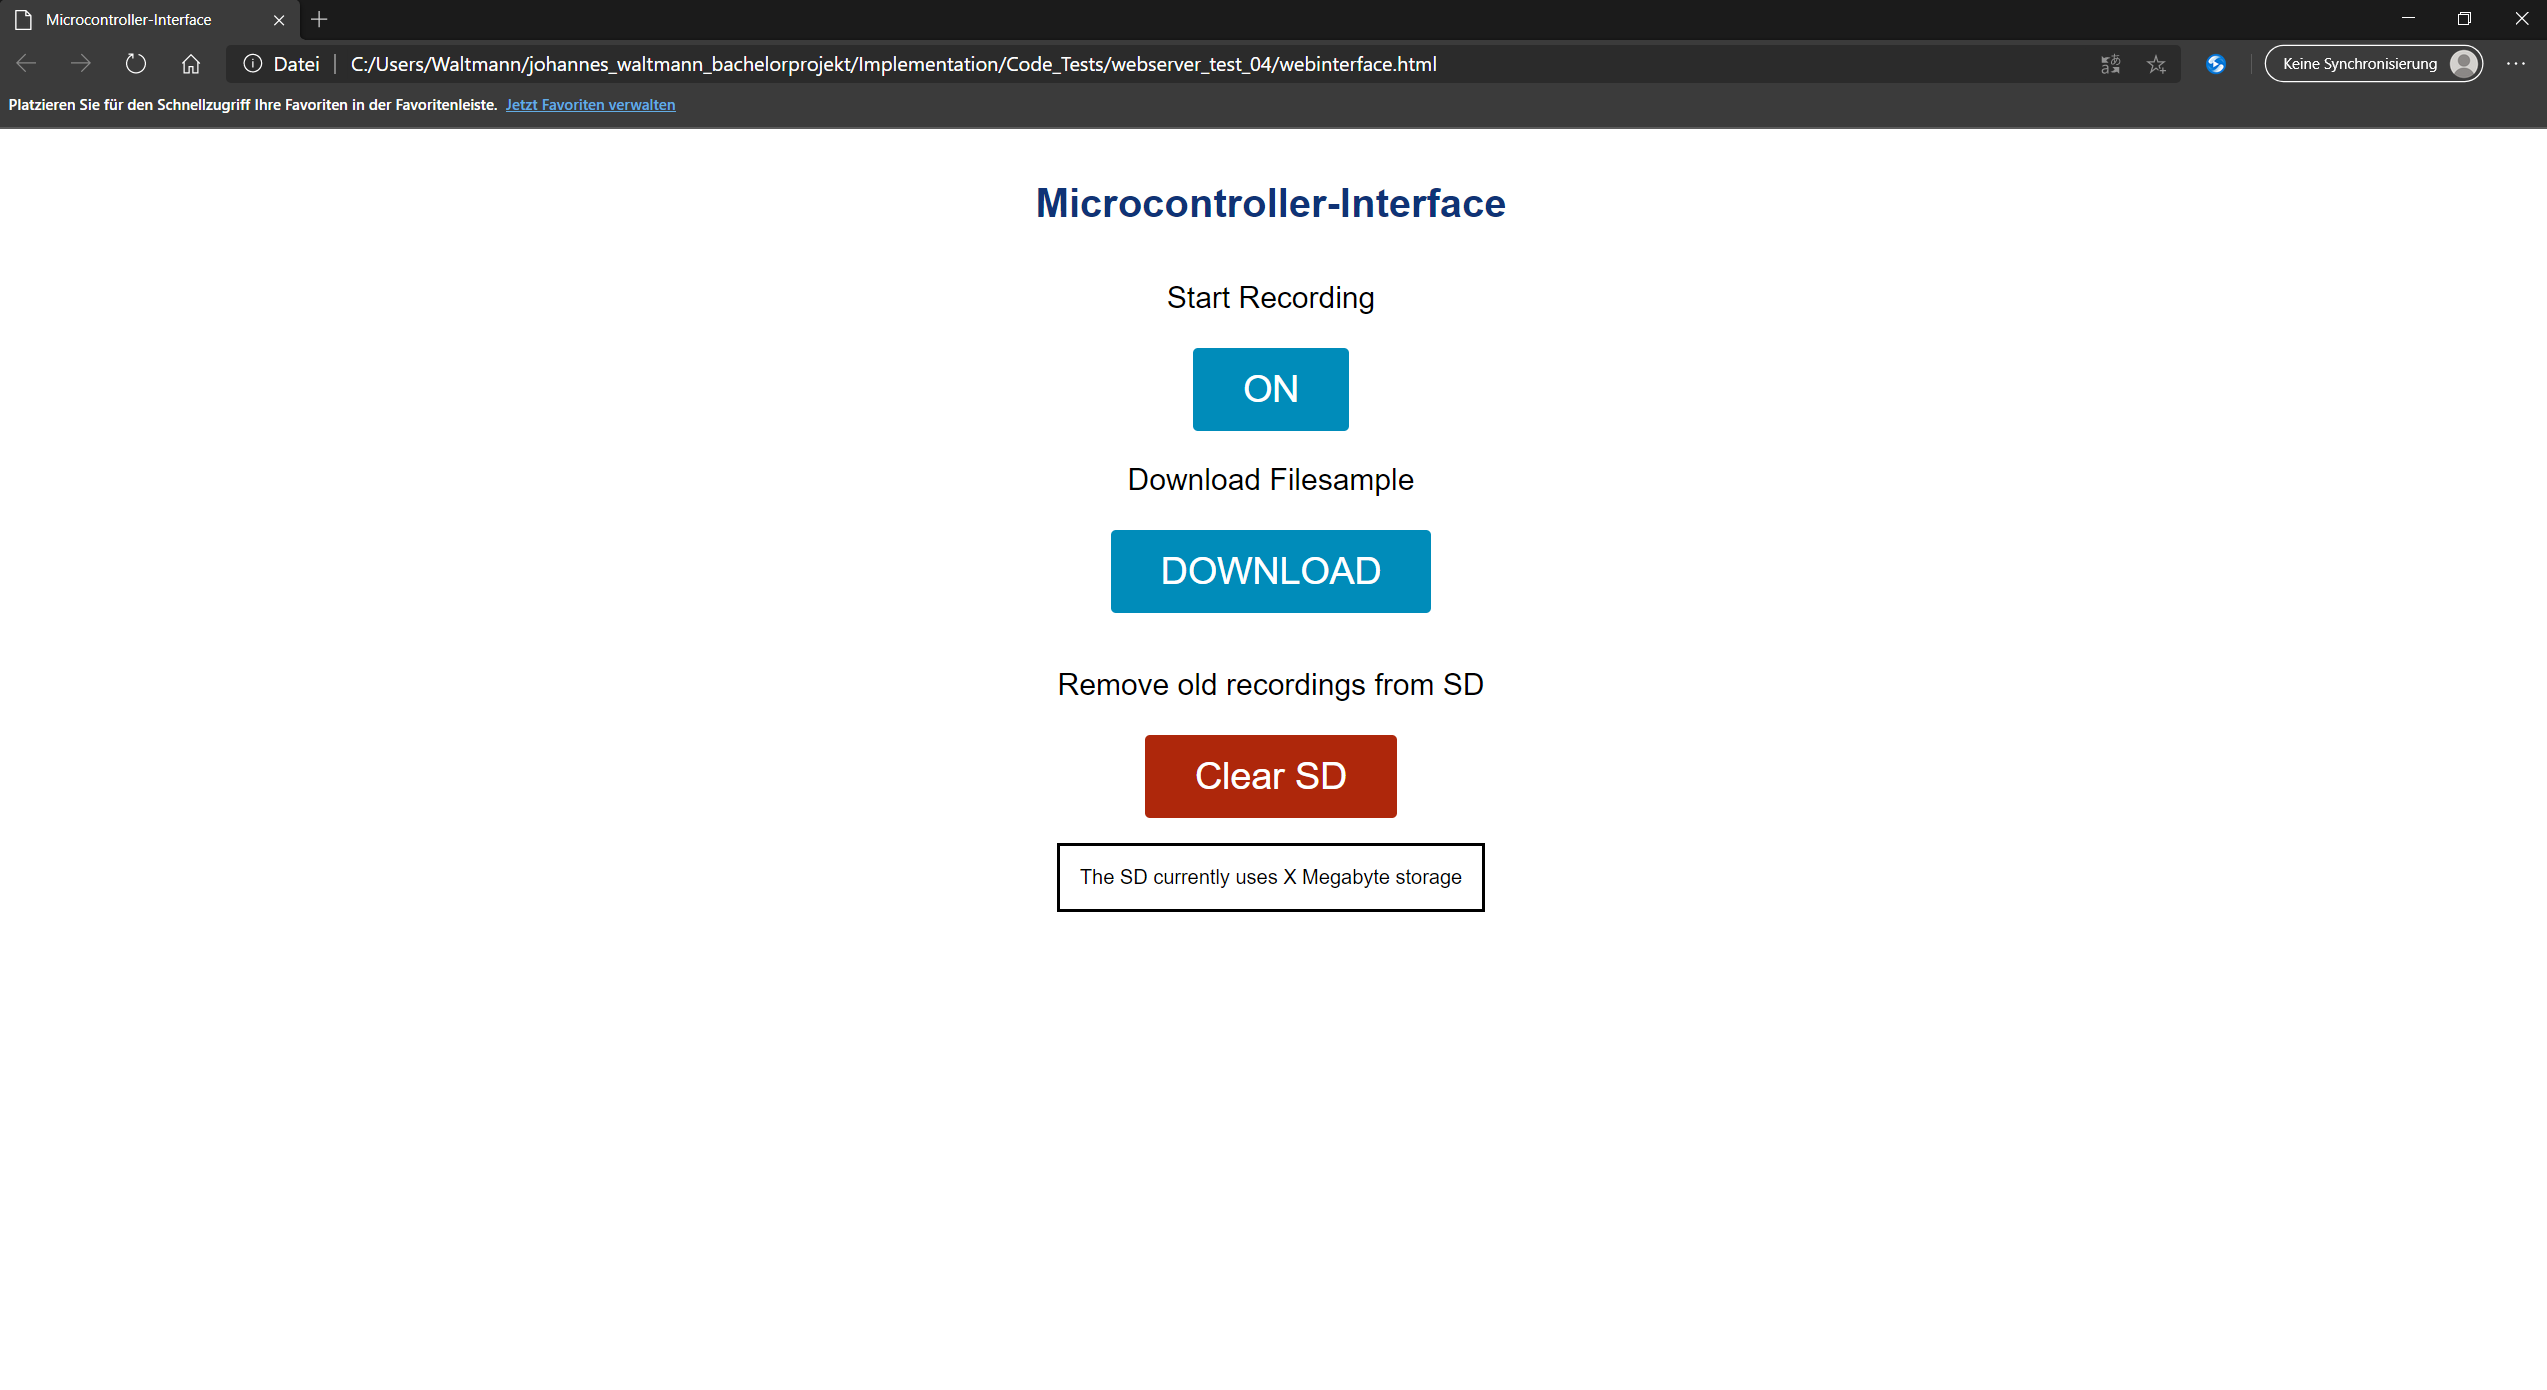
\includegraphics[width=\linewidth]{Media/webinterface_edge.png}}
	\caption{The Webinterface which is used to control the functions of the prototype as it is displayed by the Microsoft Edge browser.}
	\label{fig:webinterface}
\end{figure}
Through the interface it is possible to on the recording of a new test sample and also to remove every recording which is saved on the attached SD-card.
A third feature is located in the box on the pages bottom where the SD-cards space which is already in use is shown (represented by the character 'X').
The exact space is calculated by the method \texttt{getUsedSpace()} located in the requirements.cpp-file which then replaces the character 'X' on the interface. 
\begin{lstlisting}[frame=single, language={c++}, style=style,
	caption={The part of the loop-function which is used to manage the connection of a socket hosted on the microcontroller to a web-client.}, label={lst:WiFiCon},float=!htb]
void loop() {
	WiFiClient client = server.available();
	
	if (client) {
		currentTime = millis();
		previousTime = currentTime;
		String currentLine = "";
		while (client.connected() && currentTime - previousTime <= timeoutTime) {
			currentTime = millis();
			if (client.available()) {
				char c = client.read();
				header += c;
				if (c == '\n') {
					if (currentLine.length() == 0) {
						client.println("HTTP/1.1 200 OK");
						client.println("Content-type:text/html");
						client.println("Connection: close");
						client.println();
						
						// Handle incoming GET-Request
						
						// Print the content of the web page to be
						// displayed
						
						client.println();
						break;
					} else {
						currentLine = "";
					}
				} else if (c != '\r') {
					currentLine += c;
				}
			}
		}
		header = "";
		client.stop();
\end{lstlisting}

Other web-browsers which were used include Google Chrome and Mozilla Firefox with the latter one being the browser used most for testing the prototypes functionalities.

\section{Evaluation}
\subsection{Studydesign}
repeated measures
5-6 probanden mit je mind 2 Sessions aka 2 Tage
Alle machen das gleiche 

Armband an verscheidene Stellen
LO, LU RO RU
Tonfolge benötigt 
1x radom 1x hoch 1x tief

Jede Messung 2x machen
--> 24 measures pP

\section{Conclusion}
